% \subsubsection{Magnetic structure of the Galaxy}

% \begin{figure}[ht]
% 	\centering
% 	\begin{subfigure}{0.7\textwidth}
% 	    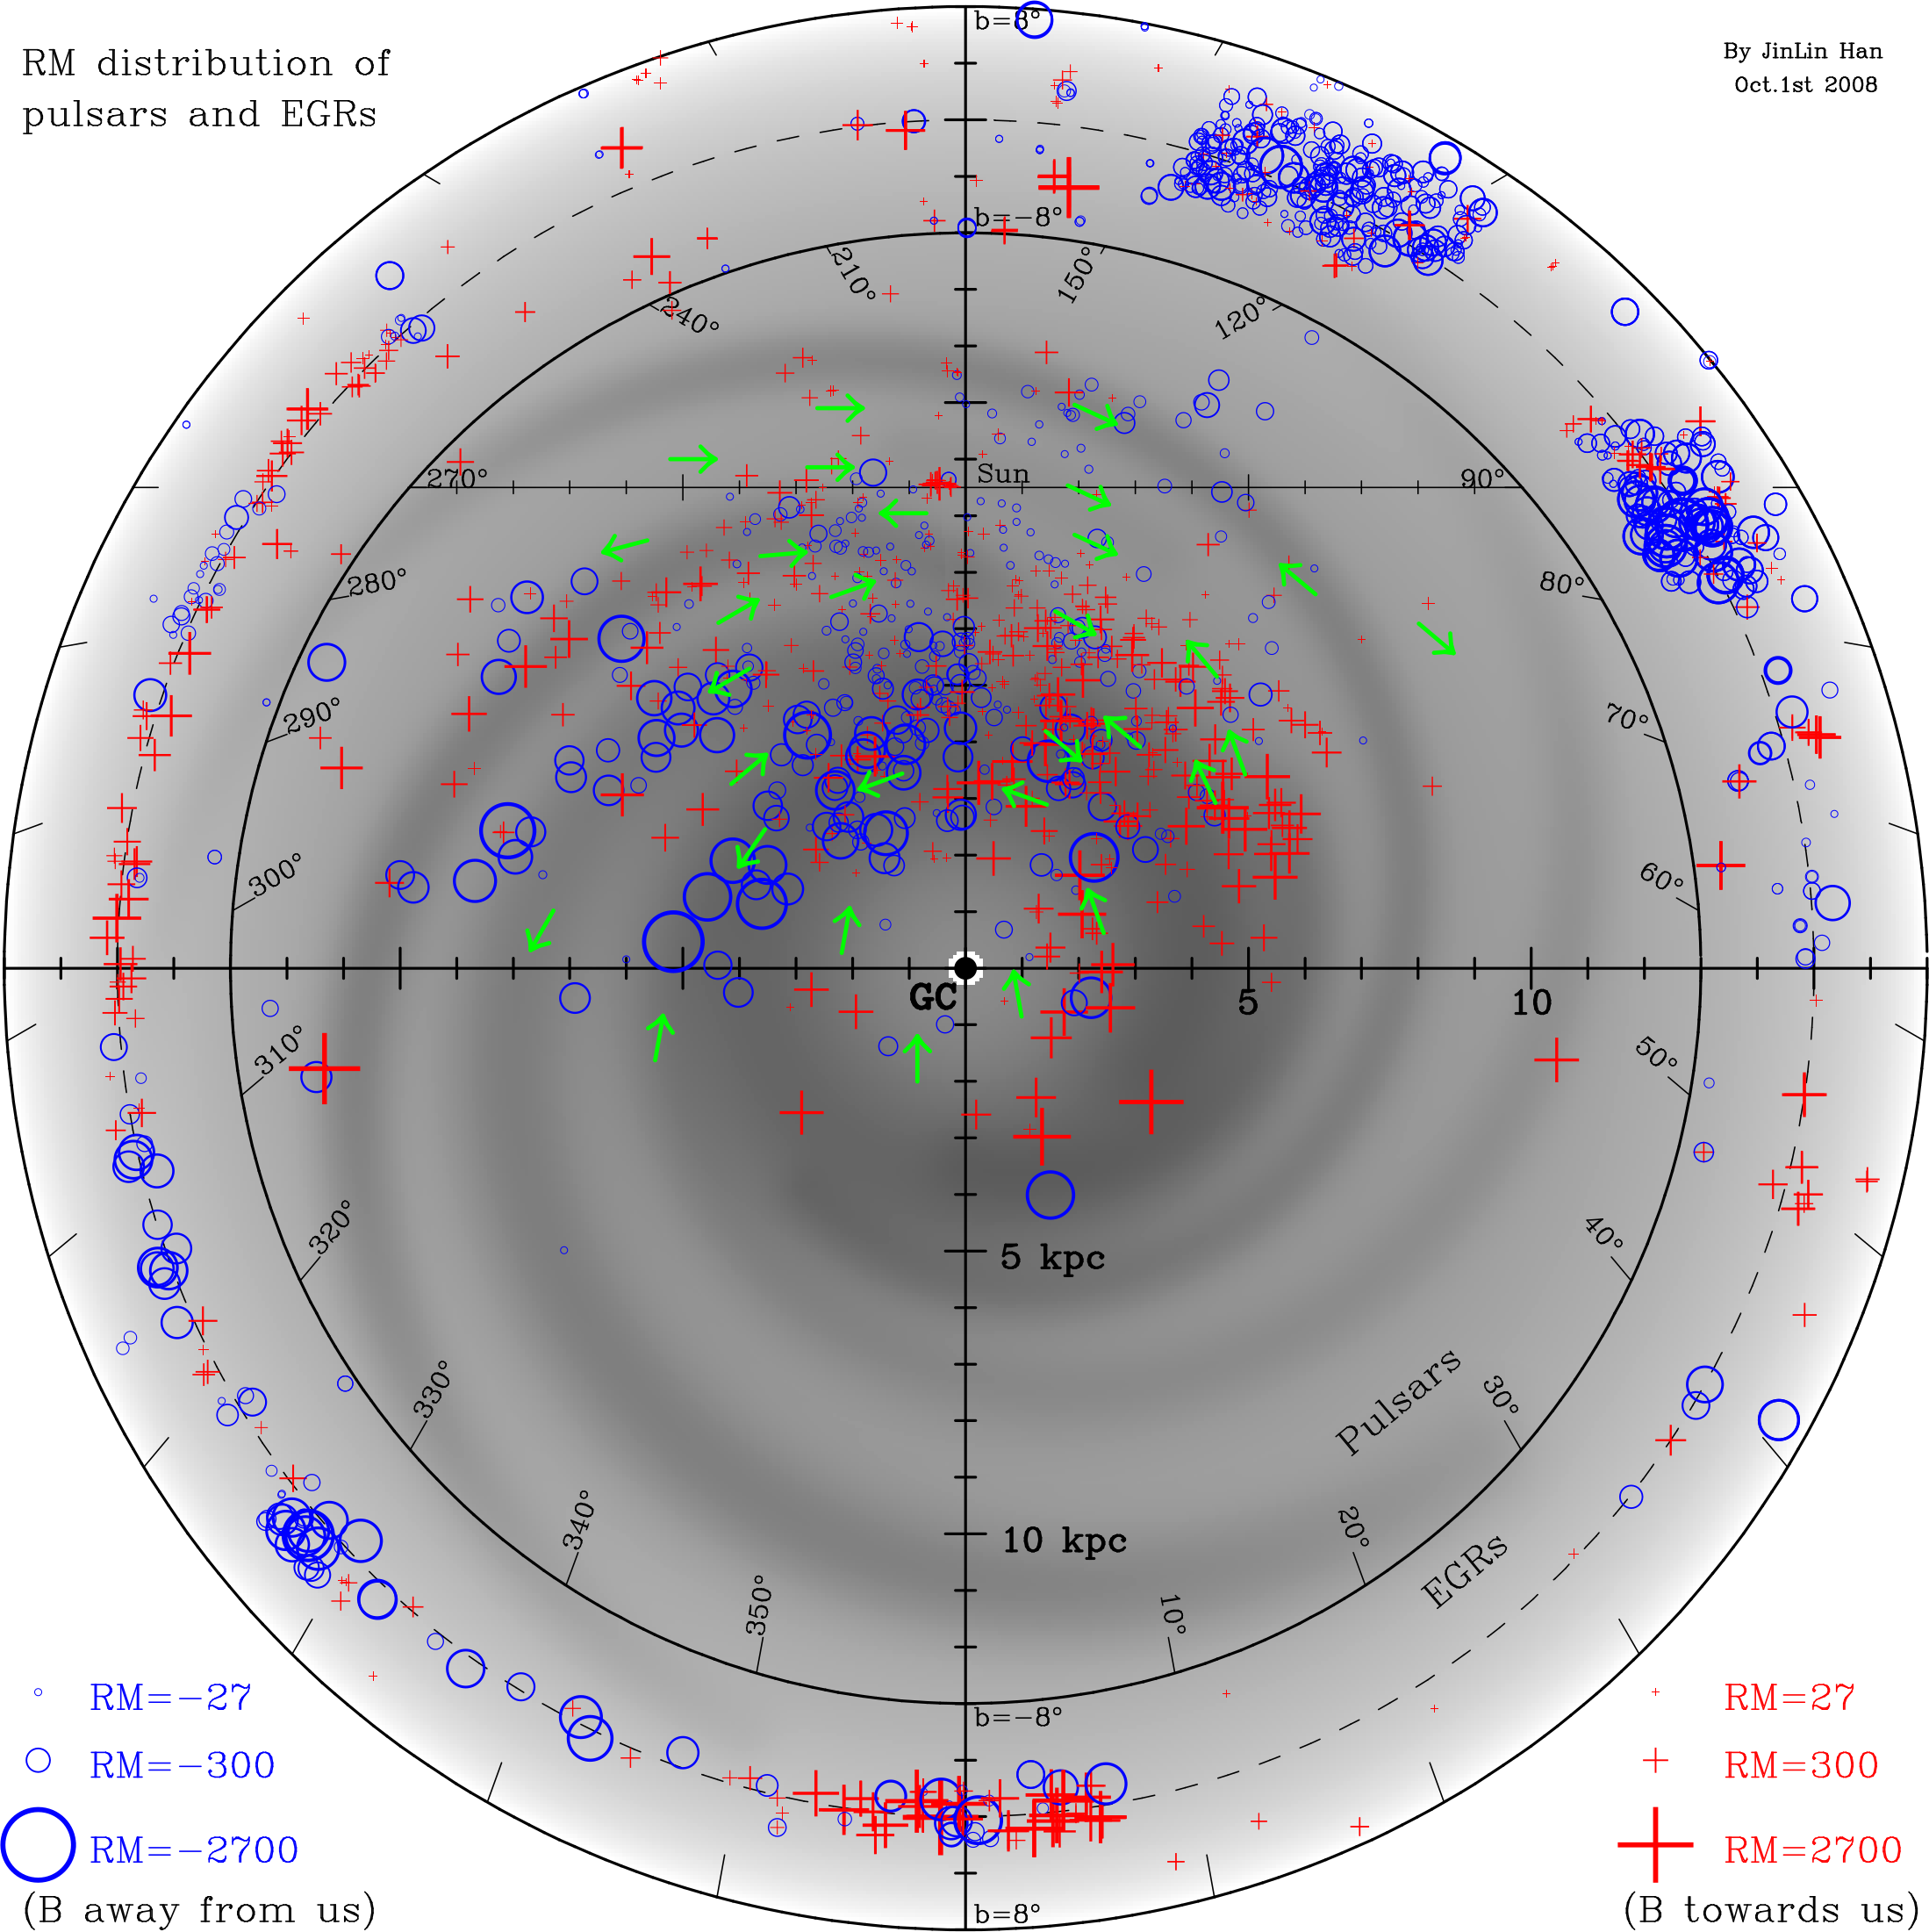
\includegraphics[width=\linewidth]{04_Introduction/Images/cosmic_rays/magnetic_field_disk.png}
% 	\end{subfigure}
% 	\begin{minipage} {0.29\textwidth}
% 	    \caption{The magnetic field structure of our Galaxy based on pulsar rotation measurements (RM). Red crosses and blue circles represent RM (i.e. magnetic field) towards and away from the Sun respectively. The structure of the magnetic field is shown by the green arrows. Image courtesy of \cite{2009IAUS..259..455H}.}
%     	\label{fig:chapter1_magnetic_structure_Galaxy}
% 	\end{minipage}
% \end{figure}

% \autoref{chapter_1_cr_propagation} showed that magnetic fields affect the propagation of cosmic rays. This subsection will briefly describe the magnetic field structure of the galaxy.
% \par~\par
% The Galactic magnetic field can be subdivided into three components; the Galactic center, the disk and the halo (the spherical component of the Galaxy). Within a few hundred parsecs of the \textbf{Galactic center}, the magnetic field has a poloidal structure with magnetic field strength of approximately $10~\si{\micro G}$ \citep{2009A&A...505.1183F}. In dense interstellar clouds, the magnetic field can be as high as $1~\si{\milli G}$ \citep{2009A&A...505.1183F}. Non-thermal radio filaments have been observed perpendicular to the magnetic plane, where the magnetic field is aligned along the filament with a strength of around $1~\si{\milli G}$.
% \par~\par
% The \textbf{Galactic disk} has a spiral like structure and contains the majority of the gas and dust in our Galaxy. Dense gas experiences amplification of magnetic fields in a manner described by Crutcher's relationship (this will be explained in \textcolor{red}{REFERENCE THIS LATER}). Faraday Rotation, the rotation of polarised electromagnetic light due to propagation in magnetised plasma \citep{1846RSPT..136....1F}, gives gives astronomers a method to determine the magnetic field strength in the line of sight:

% \begin{equation}
%     \begin{aligned}
%     \langle B_\parallel \rangle = 1.232 \frac{RM}{DM}
%     \end{aligned}
% \end{equation}
% \noindent where RM is the rotation measure due to Faraday rotation and DM is the dispersion measurement of the pulsar (see \autoref{eq:chapter_1_dispersion_measurement}) \citep{10.1093/mnras/stz1060}. \autoref{fig:chapter1_magnetic_structure_Galaxy} shows the rotational measurement distribution of 736 pulsars conducted by \cite{2009IAUS..259..455H} as well as the inferred magnetic field structure in the disk. They find that magnetic field field lines tend to run azimuthally to the Galactic centre. All the inner arms have anti-clockwise magnetic field orientation as viewed from the Galactic north pole, elsewhere the orientation depends on the position in the Galaxy. The magnetic field strength was found to depend on the distance to the Galactic centre:

% \begin{equation}
%     \begin{aligned}
%         B=B_0\exp[-\frac{R-R\odot}{R_B }]
%     \end{aligned}
% \end{equation}
% where $B_0=2.1\pm 0.3~\si{\micro G}$ and $R_B=8.5\pm 4.7~\kpc$.
% \par~\par 
% The \textbf{halo} of the Galaxy contains scattered old stars and globular clusters. \cite{10.1093/mnras/stz1060} conducted a rotation measure survey of the Galactic halo and found toroidal fields with reversed directions above and below the Galactic plane. The same study estimated that the magnetic field in the Galactic halo has a strength of at least $1.6~\si{\micro G}$. 

%Gammaray Astronomy